\documentclass[12pt, a4paper]{article}

\usepackage{array}
\usepackage[portuguese]{babel}
\usepackage{float}
\usepackage[a4paper, margin=2cm]{geometry}
\usepackage{graphicx}
\usepackage{hyperref}
\usepackage{pdfpages}
\usepackage{setspace}

\title{\textbf{Interface Pessoa-Máquina \\ \large Trabalho Prático -- Fase II}}
\date{4 de maio de 2025}
\author{Grupo 12 \\
    \url{https://github.com/UMinho-ENGINF-IPM/trabalho-pr-tico-gp25_12}}

\begin{document}

\begin{center}
    
\includegraphics[width=0.25\textwidth]{res/cover/school-of-engineering.eps}
\end{center}

{\let\newpage\relax\maketitle}
\maketitle
\thispagestyle{empty}

\chardef\_=`_
\onehalfspacing
\setlength{\parskip}{\baselineskip}
\setlength{\intextsep}{2\baselineskip}
\setlength\belowcaptionskip{-\baselineskip}
\setlength{\parindent}{0pt}
\def\arraystretch{1.5}

\vspace{2cm}
\begin{center}
    \begin{tabular}{>{\centering}p{0.25\textwidth}
                    >{\centering}p{0.25\textwidth}
                    >{\centering\arraybackslash}p{0.25\textwidth}}
        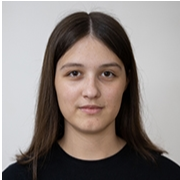
\includegraphics[width=3.5cm]{res/cover/A104437.png} &
        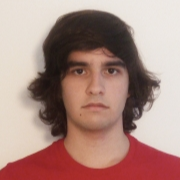
\includegraphics[width=3.5cm]{res/cover/A104348.png} &
        
\includegraphics[width=3.5cm]{res/cover/A104263.png}  \\

        Ana Oliveira & Humberto Gomes & Inês Marques \\
        A104437      & A104348        & A104263
    \end{tabular}

    \begin{tabular}{>{\centering}p{0.25\textwidth}
                    >{\centering\arraybackslash}p{0.25\textwidth}}
        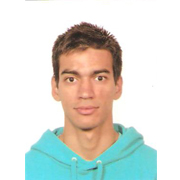
\includegraphics[width=3.5cm]{res/cover/A76350.jpg} &
        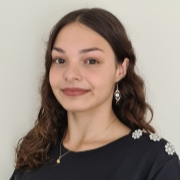
\includegraphics[width=3.5cm]{res/cover/A104179.png} \\

        Rafael Vilas Boas & Sara Lopes \\
        A76350            & A104179
    \end{tabular}
\end{center}

\begin{abstract}
    \noindent
\end{abstract}

\section{Alterações ao Modelo da Interface}

Na fase anterior deste trabalho prático, construiu-se, em Figma \cite{figma}, um modelo da interface
a implementar. Apesar de uma boa avaliação nesta fase, a docência da UC de Interface Pessoa-Máquina
reparou em alguns aspetos que podiam ser melhorados. Nesta secção, apresentam-se as mudanças que
foram feitas ao modelo da interface devido tanto aos comentários dos docentes como a outros aspetos
que o grupo de trabalho se apercebeu que podiam ser melhorados.

Em primeiro lugar, a página ``Iniciar Sessão'' não é ideal para a prevenção de erros: é possível que
o utilizador submeta parcialmente as suas credenciais (apenas o seu endereço eletrónico ou apenas a
sua palavra-passe), e o sistema reagirá com um erro. Para prevenir este erro, deve ser impossível
que um utilizador submeta as suas credenciais até as escrever todas. Logo, na nova versão do modelo
da interface, o botão de submissão de credenciais encontra-se desativado até o utilizador escrever
tanto o seu endereço eletrónico como a sua palavra-passe, como mostra a figura abaixo:

{\color{red} TODO - figura}

É importante que o utilizador saiba por que este botão se encontra desativado, pelo que, tal como
foi feito em outros botões na interface, uma \emph{tooltip} foi utilizada para justificar por que
não é possível interagir com o botão:

{\color{red} TODO - figura}

Ademais, na página ``Resolver Problemas'', o título da página foi removido, e substituído por uma
barra de pesquisa. Em primeiro lugar, o título da página não era necessário, visto que o utilizador
já sabe em que página se encontra olhando para a hiperligação realçada na barra de navegação.
Depois, o espaço que se ganha na barra lateral com a remoção deste título pode ser usado uma barra
de pesquisa, um elemento muito útil para procurar alunos em grandes listas de problemas (o cenário 1
aponta para 45 alunos sem turnos atribuídos).

{\color{red} TODO - figura}

Por último, uma sugestão da docência de Interface Pessoa-Máquina foi a eliminação da página
``Publicar Horários'', sendo estes atualizados sempre que o diretor de curso faz uma alteração. No
entanto, não consideramos esta solução viável, visto que o diretor de curso pode desejar colocar os
horários dos alunos em estados intermédios sem que estes os vejam. Por exemplo, pode desejar remover
vários alunos dos seus turnos, para os adicionar a outros turnos da mesma UC, assim, por exemplo,
abrindo vagas em turnos mais procurados. No entanto, reparou-se que é importante realçar quando as
mudanças feitas pelo diretor de curso ainda não são públicas. Por esse motivo, tal como foi feito
para o ícone de notificações, quando há alterações por publicar, um pequeno círculo é adicionado ao
canto superior direito da hiperligação para a página "Publicar Horários", como mostra a figura
abaixo:

{\color{red} TODO - figura}

\section{Componentes Implementados}

\section{Páginas Implementadas}

\section{Tecnologias Utilizadas}

Para a realização deste projeto, foi necessário o uso de diversas tecnologias. Nesta secção,
procura-se apresentar as diversas tecnologias utilizadas, como estas foram utilizadas, e as
facilidades e dificuldades sentidas com cada uma.

\subsection{HTML e CSS}

Visto que a aplicação desenvolvida é uma aplicação Web, o uso de HTML e CSS é imperativo em quase
todas as \emph{frameworks}. De um modo geral, o desenvolvimento de componentes e páginas com recurso
a estas tecnologias foi fácil, especialmente devido à sua natureza declarativa. Outra facilidade do
uso destas tecnologias foram as flexboxes, que simplificaram a organização dos elementos nas
componentes e nas páginas.

No entanto, houve algumas dificuldades em garantir que o código desenvolvido funcionava em todos os
navegadores: como nem todos os navegadores suportavam todas as funcionalidades desejadas, foi
necessário testar a aplicação desenvolvida em Chromium (Blink), Firefox (Gecko) e Safari (WebKit).
Várias vezes, foi necessário adicionar regras de CSS com \emph{vendor prefixes}, ou até refazer
algumas funcionalidades devido a diferenças de funcionamento entre navegadores.

\subsection{TypeScript}

\hyphenation{Java-Script}

No projeto desenvolvido, foi utilizado TypeScript \cite{typescript}, linguagem que é transpilada
para JavaScript, mas que permite alguma verificação de tipos. O TypeScript foi uma grande ajuda para
garantir a correção do código da aplicação, e assegurar, em \emph{compile-time}, que a aplicação não
terá exceções em \emph{runtime} devido a erros de tipos. Ademais, o compilador não obriga que o
código seja tipado durante o processo de desenvolvimento, pelo que este pode continuar a ser
bastante veloz. Assim, apenas quando se acaba de escrever um módulo / componente / página, podem
adicionar-se anotações de tipo ao código para garantir a sua correção.

\subsection{Vue}

A \emph{framework} utilizada para o desenvolvimento da aplicação foi Vue.js \cite{vue}. Esta
\emph{framework}, devido à sua natureza declarativa e reativa, foi de muito fácil atualização:
alterar um objeto reativo conduzia à atualização automática das partes da componente / página que
sofreram alterações. Por exemplo, ao contrário do Blazor \cite{blazor}, utilizado em Laboratórios de
Informática IV, não era necessário chamar uma função (\texttt{StateHasChanged}) sempre que era
necessário atualizar os conteúdos da DOM.

Apesar de poucas, foram sentidas algumas dificuldades no uso de Vue, especialmente quando era
necessário integrar funcionalidades não reativas (no caso, a resposta a um evento de mudança de uma
\emph{media query}) com a reatividade do Vue, tendo sido necessários \emph{hacks} para forçar a
atualização dos objetos reativos.

\subsection{Pinia}

A biblioteca Pinia \cite{pinia} foi utilizada para armazenamento do estado da aplicação, como as
credenciais do utilizador, o tema da aplicação (claro ou escuro) e os turnos escolhidos nas páginas
``Horário Completo'' e ``Gerir Turnos'', para que esta informação não desapareça quando se navega
entre diferentes páginas da aplicação. Adicionalmente, o \emph{plugin}
\texttt{pinia-plugin- persistedstate} \cite{pinia-persistent} foi utilizado para persistir algum
estado no \texttt{localStorage} do navegador, para este ser mantido mesmo após o navegador ser
fechado. Por exemplo, as credenciais do utilizador são armazenadas no \texttt{localStorage} quando
este escolhe que deseja que a aplicação se ``lembre de si''.

O Pinia, devido à sua integração com Vue, foi das ferramentas de mais fácil utilização, visto que os
objetos armazenados nos \emph{stores} do Pinia podiam ser utilizados como qualquer outro objeto
reativo do Vue.

\subsection{JSON Server}

É necessário que a aplicação desenvolvida tenha dados que possa apresentar. Na UC de Interface
Pessoa-Máquina, não é pedido que se implemente um \emph{backend} completo para a aplicação, pelo que
se utilizou \texttt{json-server} \cite{json-server}, um programa que cria uma API REST a partir dos
dados num ficheiro JSON.

A utilização desta tecnologia foi complicada, não devido a complexidade da tecnologia em si, mas sim
devido ao trabalho necessário para organizar os dados da API num formato adequado para apresentação.
Devido às capacidades muito limitadas de interrogação do \texttt{json-server}, várias interrogações
tiveram de ser implementadas imperativamente em JavaScript, ao contrário de declarativamente numa
linguagem especializada, como se teria feito caso se tivesse utilizado uma base de dados. O uso de
uma base de dados seria, por este motivo, uma grande melhoria ao projeto.

\subsection{Outras tecnologias}

O \texttt{npm} \cite{npm} é o gestor de pacotes do NodeJS, que permite, no ficheiro
\texttt{pacakage.json}, definir as dependências do projeto desenvolvido. Além disso, também é
possível definir \emph{scripts} como \texttt{npm run dev}, para abrir a aplicação com ferramentas de
desenvolvimento, e \texttt{npm run preview}, para pré-visualização da aplicação final. Para melhorar
a experiência de desenvolvimento, estes dois \emph{scripts} foram modificados para, além de
executarem o servidor HTTP da aplicação, também executarem o JSON Server. Também foram adicionados
\emph{scripts} para, com recurso às ferramentas ESLint \cite{eslint} e Prettier \cite{prettier},
automaticamente fazer uma análise estática e formatação do código, respetivamente. Estes
\emph{scripts} são usados na \emph{pipeline} de CI (\emph{Continuous Integration}) do repositório do
projeto (GitHub Actions), obrigando a que todos os \emph{pull requests} tenham código correto e bem
formatado.

A principal dificuldade do uso do \texttt{npm} foi garantir que os \emph{scripts} criados
funcionavam em diferentes sistemas operativos, visto que alguns comandos utilizados apenas estavam
disponíveis, por exemplo, em Linux.

\section{Conclusão e Trabalho Futuro}

\begingroup
\section{Bibliografia}
\renewcommand{\section}[2]{}

\begin{thebibliography}{9}
    \bibitem{figma}
        ``Figma: Collaborative Interface Design Tool''. Figma. Accessed: Mar. 13, 2025. [Online.]
        Available: \url{https://www.figma.com/}
    \bibitem{typescript}
        ``TypeScript''. TypeScript. Accessed: Apr. 30, 2025. [Online.] Available:
        \url{https://www.typescriptlang.org/}
    \bibitem{vue}
        ``The Progressive JavaScript Framework''. Figma. Accessed: Apr. 30, 2025. [Online.]
        Available: \url{https://vuejs.org/}
    \bibitem{blazor}
        `` Launch your idea to the web fast with Blazor''. Blazor. Accessed: Apr. 30, 2025.
        [Online.] Available: \url{https://dotnet.microsoft.com/en-us/apps/aspnet/web-apps/blazor}
    \bibitem{pinia}
        ``Pinia: The intuitive store for Vue.js''. Pinia. Accessed: Apr. 30, 2025. [Online.]
        Available: \url{https://pinia.vuejs.org/}
    \bibitem{pinia-persistent}
        ``Pinia Plugin Persistedstate: Configurable persistence of Pinia stores''.
        Pinia Plugin Persistedstate. Accessed: Apr. 30, 2025. [Online.] Available:
        \url{https://prazdevs.github.io/pinia-plugin-persistedstate/}
    \bibitem{json-server}
        ``json-server''. GitHub. Accessed: Apr. 24, 2025. [Online.] Available:
        \url{https://github.com/typicode/json-server}
    \bibitem{npm}
        ``NPM''. NPM. Accessed: Apr. 24, 2025. [Online.] Available: \url{https://www.npmjs.com/}
    \bibitem{eslint}
        ``ESLint''. ESLint. Apr. 24, 2025. [Online.] \url{https://eslint.org/}
    \bibitem{prettier}
        ``Prettier''. Prettier. Apr. 24, 2025. [Online.] \url{https://prettier.io/}
\end{thebibliography}
\endgroup

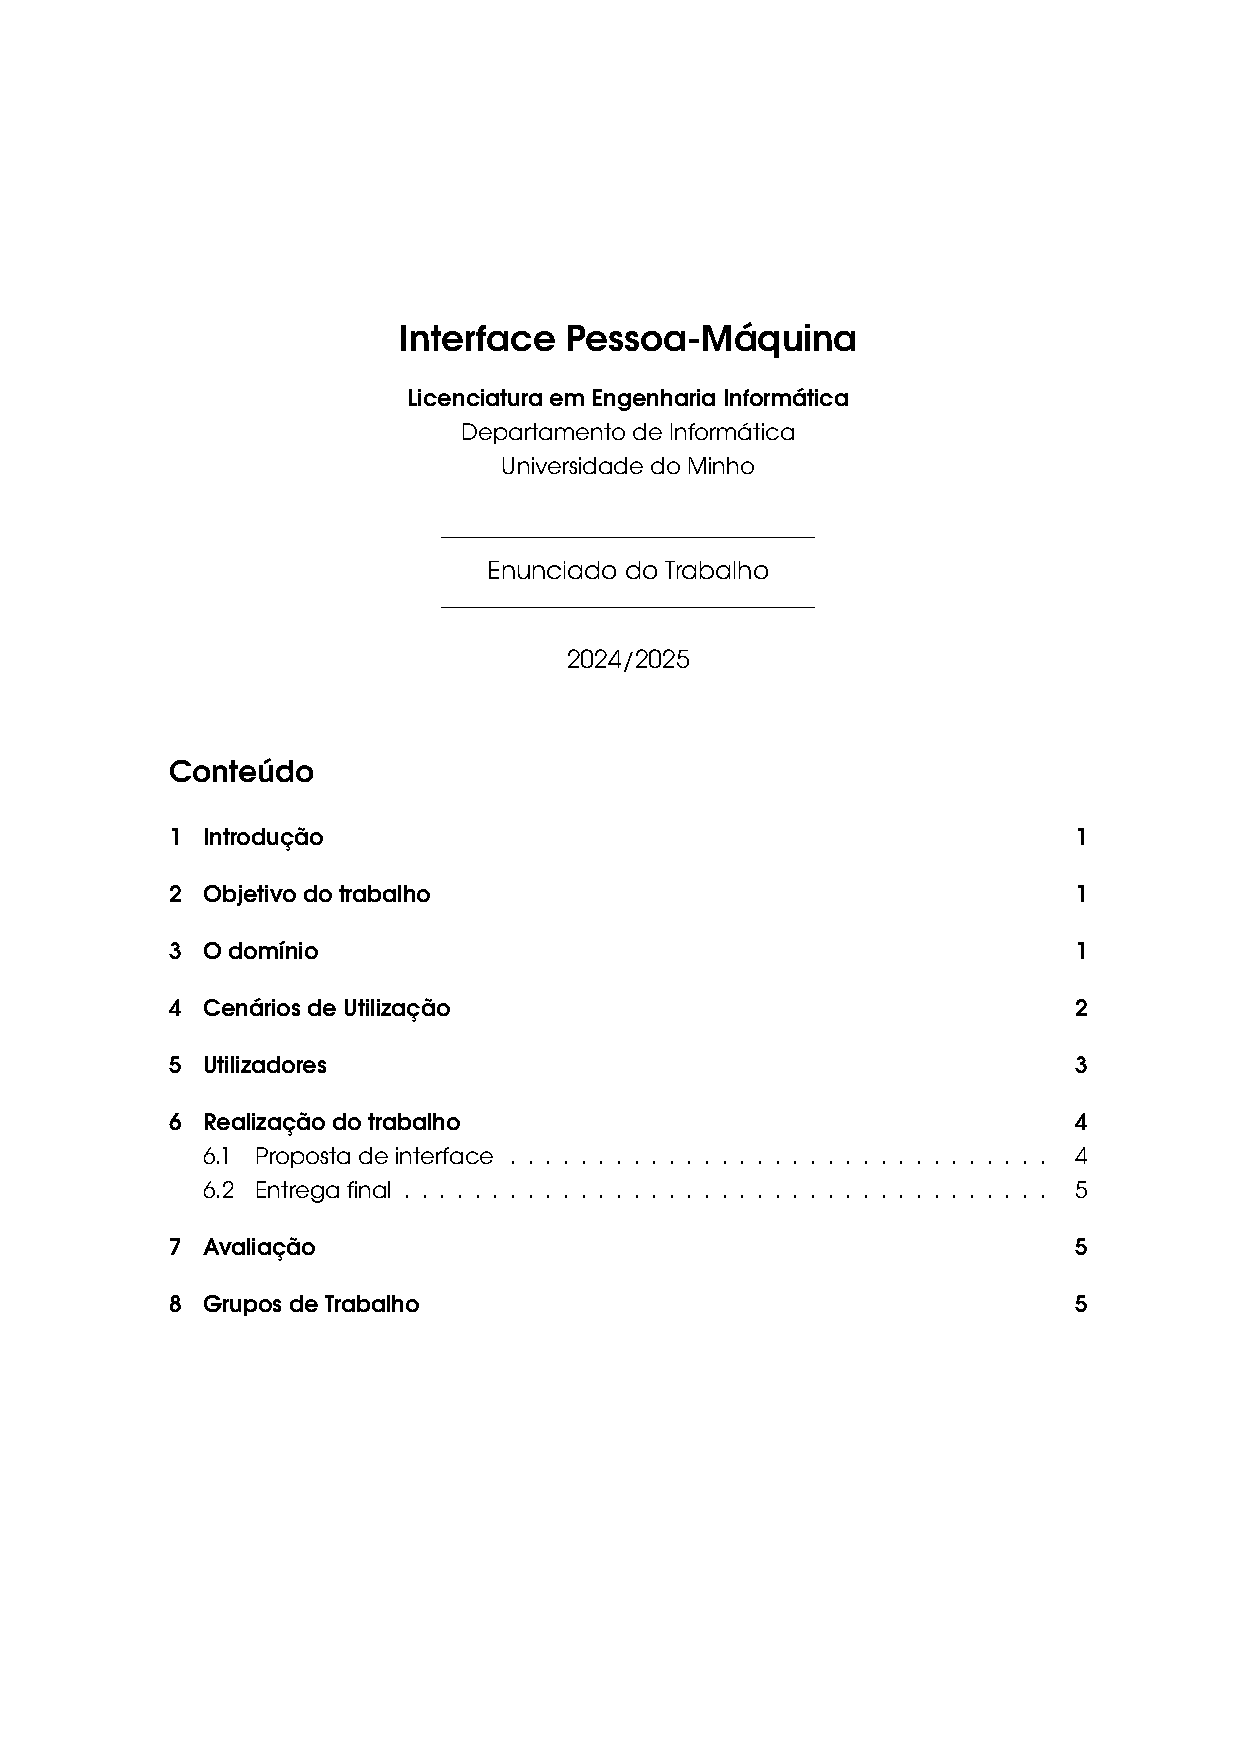
\includepdf[pages=1,pagecommand=\section{Anexo -- Enunciado do Trabalho}\thispagestyle{empty}]
    {../Assignment.pdf}
\includepdf[pages=2-]{../Assignment.pdf}

\end{document}
